\documentclass{scrartcl}

\usepackage[linear]{handout}
\usepackage{bbm}
\usepackage{circuitikz}
% \usepackage{mlmodern}
% \usepackage{gfsartemisia}
\ihead{\sffamily\bfseries\footnotesize{Experiment 01}}
\ohead{\sffamily\footnotesize\textbf{}} 

\title{
        \Large\textsc{PH3204: Electronics Lab} \\
        \vspace{10pt}
        % \Large\textsc{Experiment 02} \\
        % \vspace{0.1cm}
        \Huge \textbf{Study of an npn Bipolar Junction Transistor(BJT)} \\
}

% \subtitle{}

\author{Sabarno Saha \\ \texttt{22MS037} \\ Grp. B-10}

\date{\normalsize
        \textit{Indian Institute of Science Education and Research, Kolkata, \\
        Mohanpur, West Bengal, 741246, India.}
        % \vspace{10pt}
        % \today
}
\newcommand{\1}{\mathbbm{1}}
\newcommand{\ichi}{\tilde{\chi}}
\newcommand{\irho}{\tilde{\rho}}
\newcommand{\ihsr}{\tilde{H}_{SR}}
\newcommand{\G}{\Gamma}
\newcommand{\iG}{\tilde{\Gamma}}
\newcommand{\is}{\tilde{s}}
\newcommand{\h}{\mathbb{H}}
\newcommand{\nbar}{\bar{n}}

\graphicspath{{./code/}}

\begin{document}
\maketitle
\tableofcontents
\section{Aim}

The aim of this experiment is two fold, we want to study the input and output characteristics of an npn
Bipolar Junction Transistor (BJT) and also to determine the current gain of the BJT.

\begin{itemize}
	\item To study the input characteristics of an npn BJT.
	\item To study the output characteristics of an npn BJT.
	\item To determine the current gain of the BJT.
\end{itemize}



\section{Theory}
The Bipolar Junction Transistor(BJT) used in the amplifications of signals and also as switches in circuits. There are two types of BJT, namely , npn and pnp. In this experiment we will be studying the npn BJT.
 The npn BJT consists of three layers of semiconductors, namely, the emitter, base and collector. The emitter is heavily doped, the base is lightly doped and the collector is moderately doped. 
 The BJT has two junctions, the emitter-base junction and the collector-base junction. 

The BJT can be used in many different configurations, here we will study it in the Common Emitter(CE) configuration. In this configuration, the input is given to the base and the output is taken from the collector. 
The emitter is common to both the input and output. 
The input characteristics of the BJT is the plot of the base current($I_b$) vs the base-emitter voltage($V_{BE}$) for a fixed collector voltage($V_{CC}$). 
The output characteristics of the BJT is the plot of the collector current($I_c$) vs the collector-emitter voltage($V_{CE}$) for a fixed base current($I_b$).

Here, we also study the current gain of the BJT. When the BJT is used as an amplififer,the base emitter junction is forward biased and the collector base junction is reverse biased. In the forward bias, the electrons flow from the 
emitter to the base and in the reverse bias, the electrons flow from the base to the collector. There is a small amount of recombination in the base region, which gives rise to the base current $I_b$. The collector current $I_c$ is
almost equal to the $I_c$ and is given by the formula:
\begin{equation}
        I_c = \alpha I_E
\end{equation}
where $\alpha$ should be close to 1. Thus the current gain is given by
\begin{equation}
        \beta = \frac{I_c}{I_b}
\end{equation}
where $\beta = \frac{\alpha}{1 - \alpha}$, which should be quite large.

The circuit we use for the experiment is given below.


\begin{figure}[H]
	\centering
	\resizebox{0.75\textwidth}{!}{
\begin{tikzpicture}
	
	% Paths, nodes and wires:
	\draw node[npn, xscale=1.41, yscale=1.41] at (8.84, 5.25) {};
	\draw (8, 5.25) to[american resistor, l={$R_B$}, label distance=0.02cm] (5, 5.25);
	\draw (3.5, 5.25) to[battery, l={$V_{BB}$}, label distance=0.02cm] (3.5, 2.75);
	\draw (7.5, 5.25) to[voltmeter, l={$V_{BE}$}, label distance=0.02cm] (7.5, 2.75);
	\draw (10, 6) to[voltmeter, l={$V_{CE}$}, label distance=0.02cm] (10, 2.75);
	\draw (8.84, 6.336) -| (10, 6);
	\draw (8.84, 4.164) |- (10, 2.75) -- (5, 2.75) |- (3.5, 2.75);
	\draw (3.5, 5.25) to[ammeter, l={$I_b(\mu A)$}, label distance=0.02cm] (5, 5.25);
	\draw (12.2, 6.3) to[ammeter, l={$I_c  (mA)$}, label distance=0.02cm] (13.9, 6.3);
	\draw (10, 6.3) to[american resistor, l={$R_c$}, label distance=0.02cm] (12.2, 6.3);
	\draw (13.9, 6.3) to[battery, l={$V_{cc}(V)$}, label distance=0.02cm] (13.9, 2.8);
	\draw (10, 2.75) -| (13.9, 2.8);
	\node[shape=circle, draw, line width=1pt, inner sep=0, minimum width=1.512cm] at (8.774, 5.25){};
\end{tikzpicture}}
\caption{Circuit diagram of an npn BJT.}
\end{figure}
\section{Data and Analysis}
\subsection{Input Characteristics of an npn BJT}
For this part we wish to study the input characteristic curve of the given transistor. We fix the collector to emitter voltage($V_{CE}$) and then vary
the base bias voltage($V_{BB}$) and measure the base current($I_b$). We take three Datasets for input voltage, with $V_{CC} = 2V, 3V, 4V$. The data is 
given in the Supplementary section \cref{sec:supplementary}(\cref{tab:input2v}, \cref{tab:input3v}, \cref{tab:input4v}). We plot the input characteristics below.

We set $R_B = 1 k \Omega$ and $R_C = 1 \Omega$ for this part of the experiment. For the experiment we do not put in $R_C$ at all, but the value is taken 
small enough to show that $R_c$ should be neglected.
\begin{figure}[H]
        \centering
        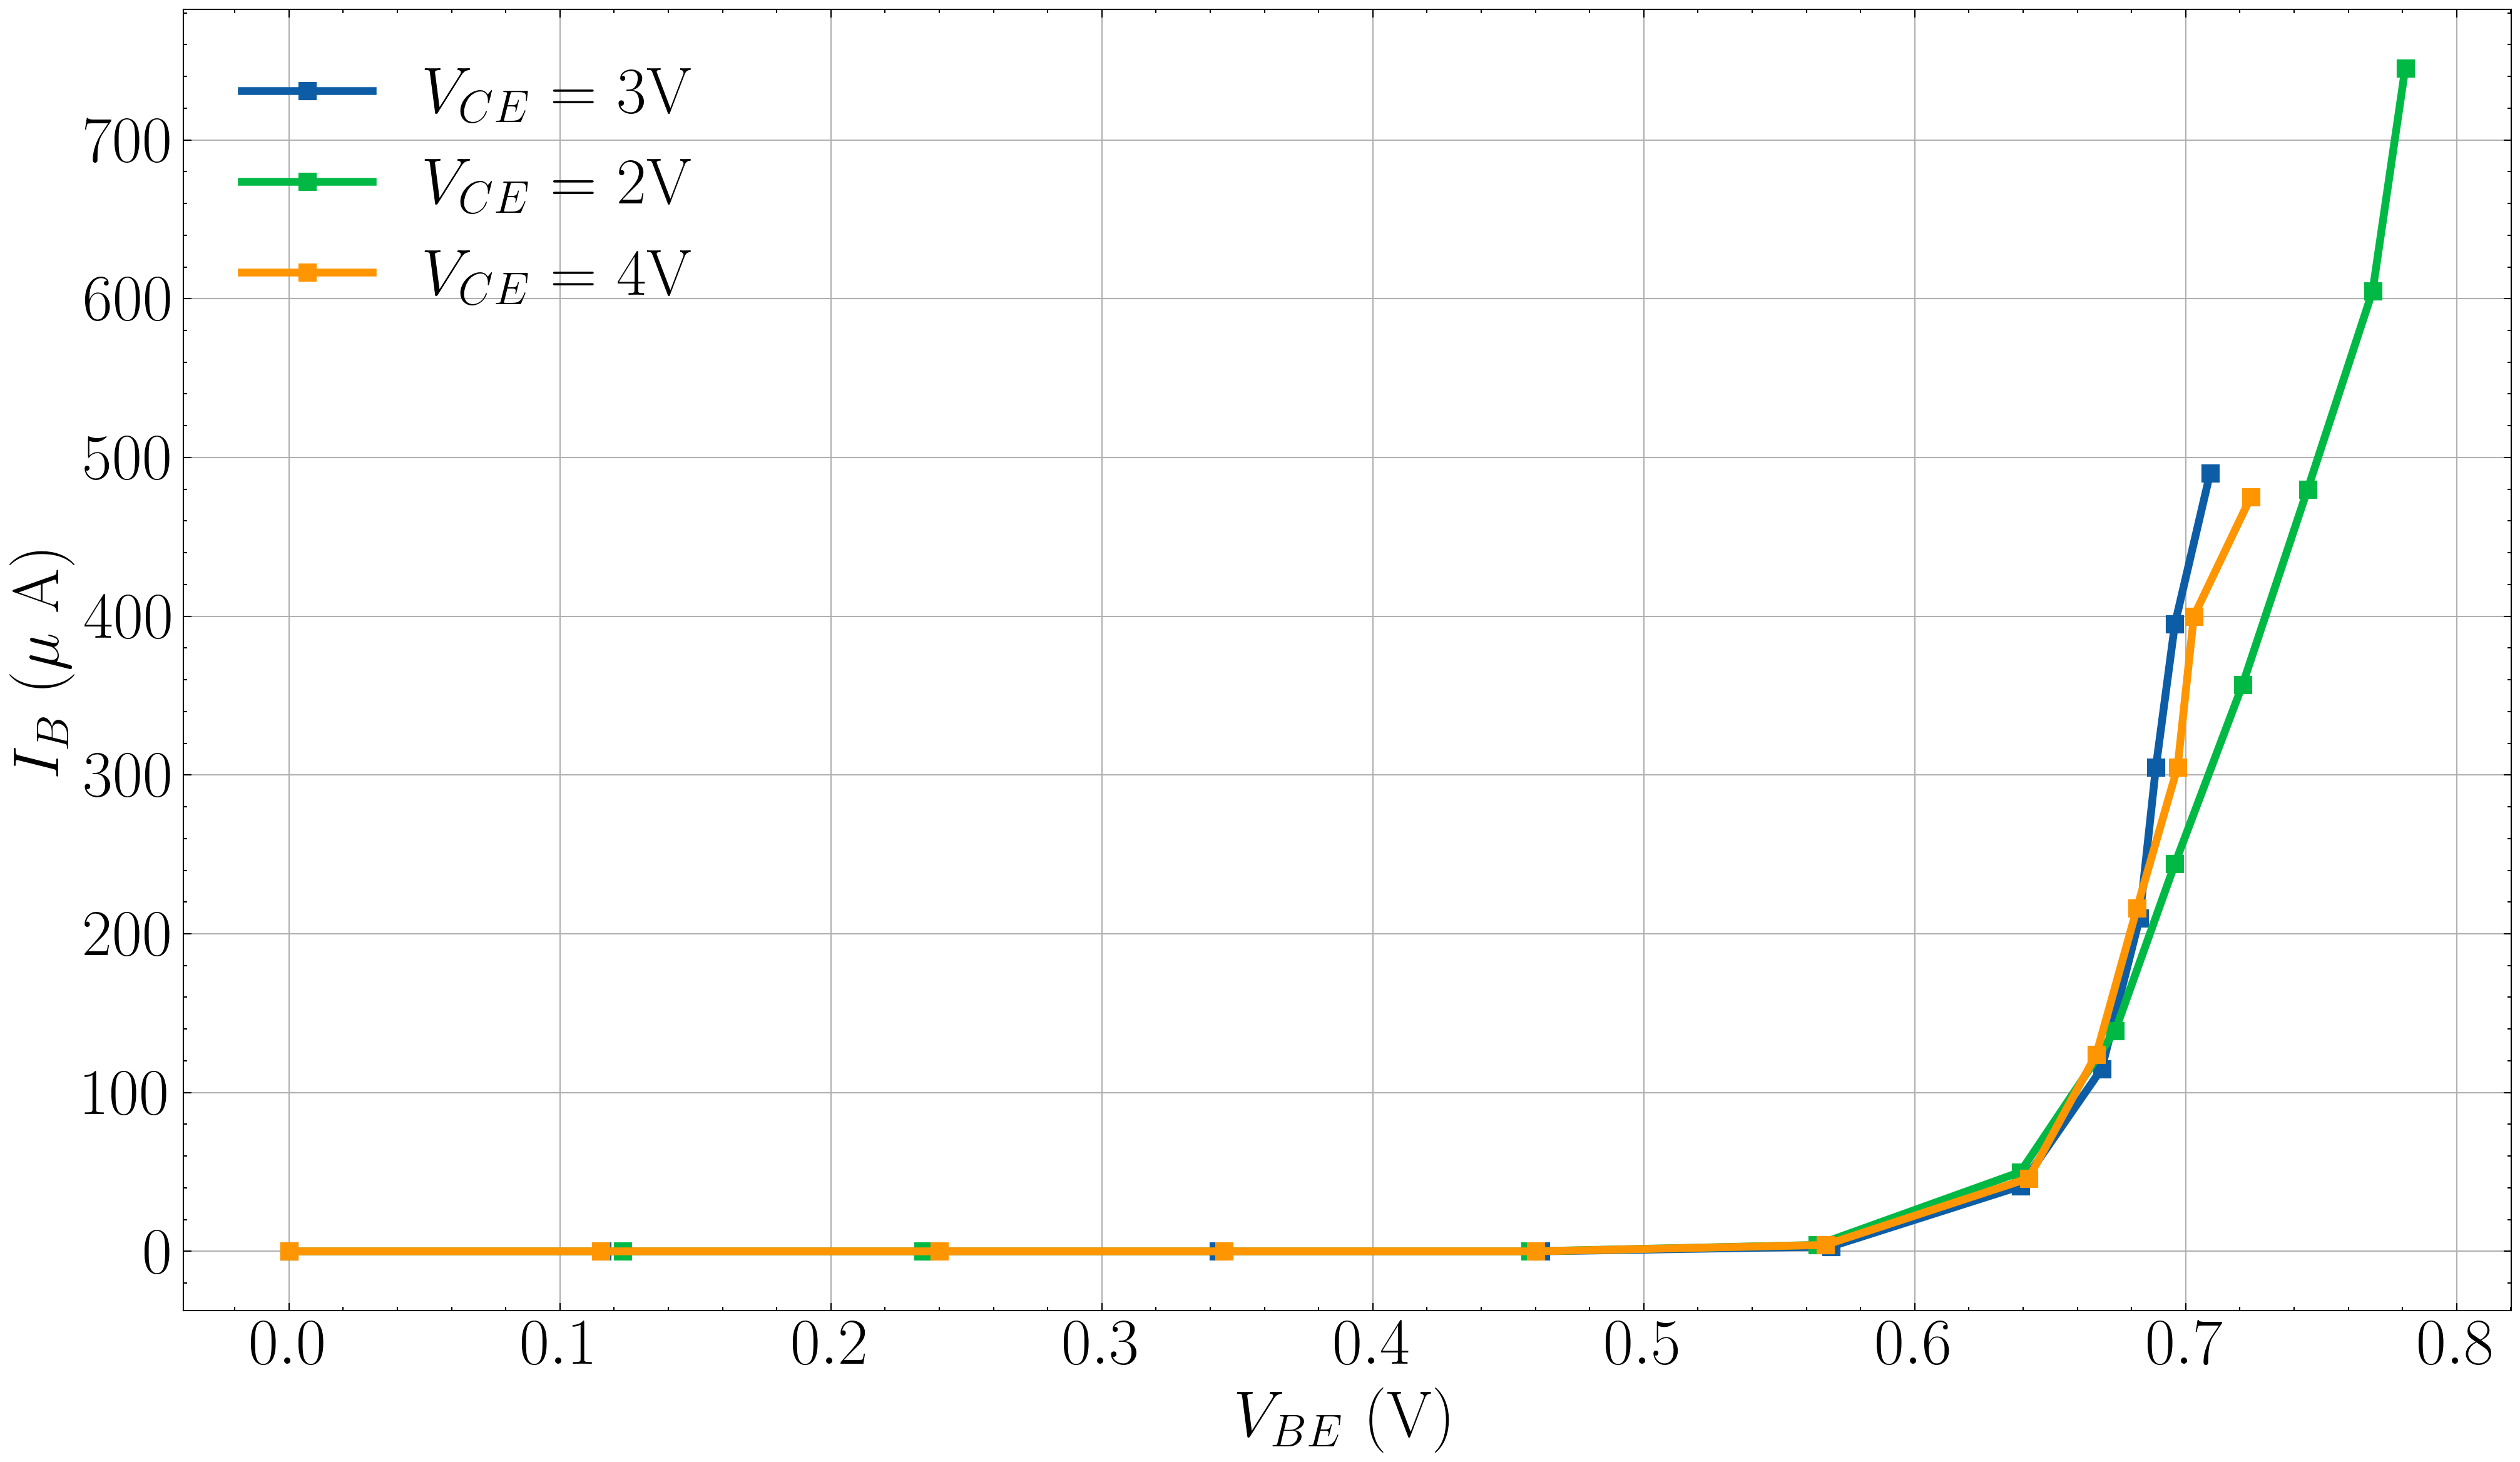
\includegraphics[width=0.75\textwidth]{input.png}
        \caption{Input Characteristics of an npn BJT}
\end{figure}
\emph{Note:} We expect the $4V$ line to be right of the $3V$ line which in turn should be in the right of the $2V$ line. However, experimentally, 
we observe something different. The $4V$ line lies to the right of the $3V$ line but both the lines lie to the left of the $2V$ line.
\subsection{Output Characteristics of an npn BJT}
For this part we wish to study the output characteristic curve of the given transistor. We fix the base current($I_b$) and then vary the collector voltage($V_{CE}$) and measure the collector current($I_c$). We take three 
 Datasets for input voltage, with $I_b = 10 \mu A, 20 \mu A, 30 \mu A$. For this experiment, we used $R_B = 220 \Omega$ and $R_C = 1 k\Omega$. The data is
 given in the Supplementary section \cref{sec:supplementary}(\cref{tab:output10}, \cref{tab:output20}, \cref{tab:output30}). We plot the output characteristics below.
We see that the plot agrees with theory, where the collector current increases with the collector-emitter voltage and then saturates.
\begin{figure}[h]
        \centering
        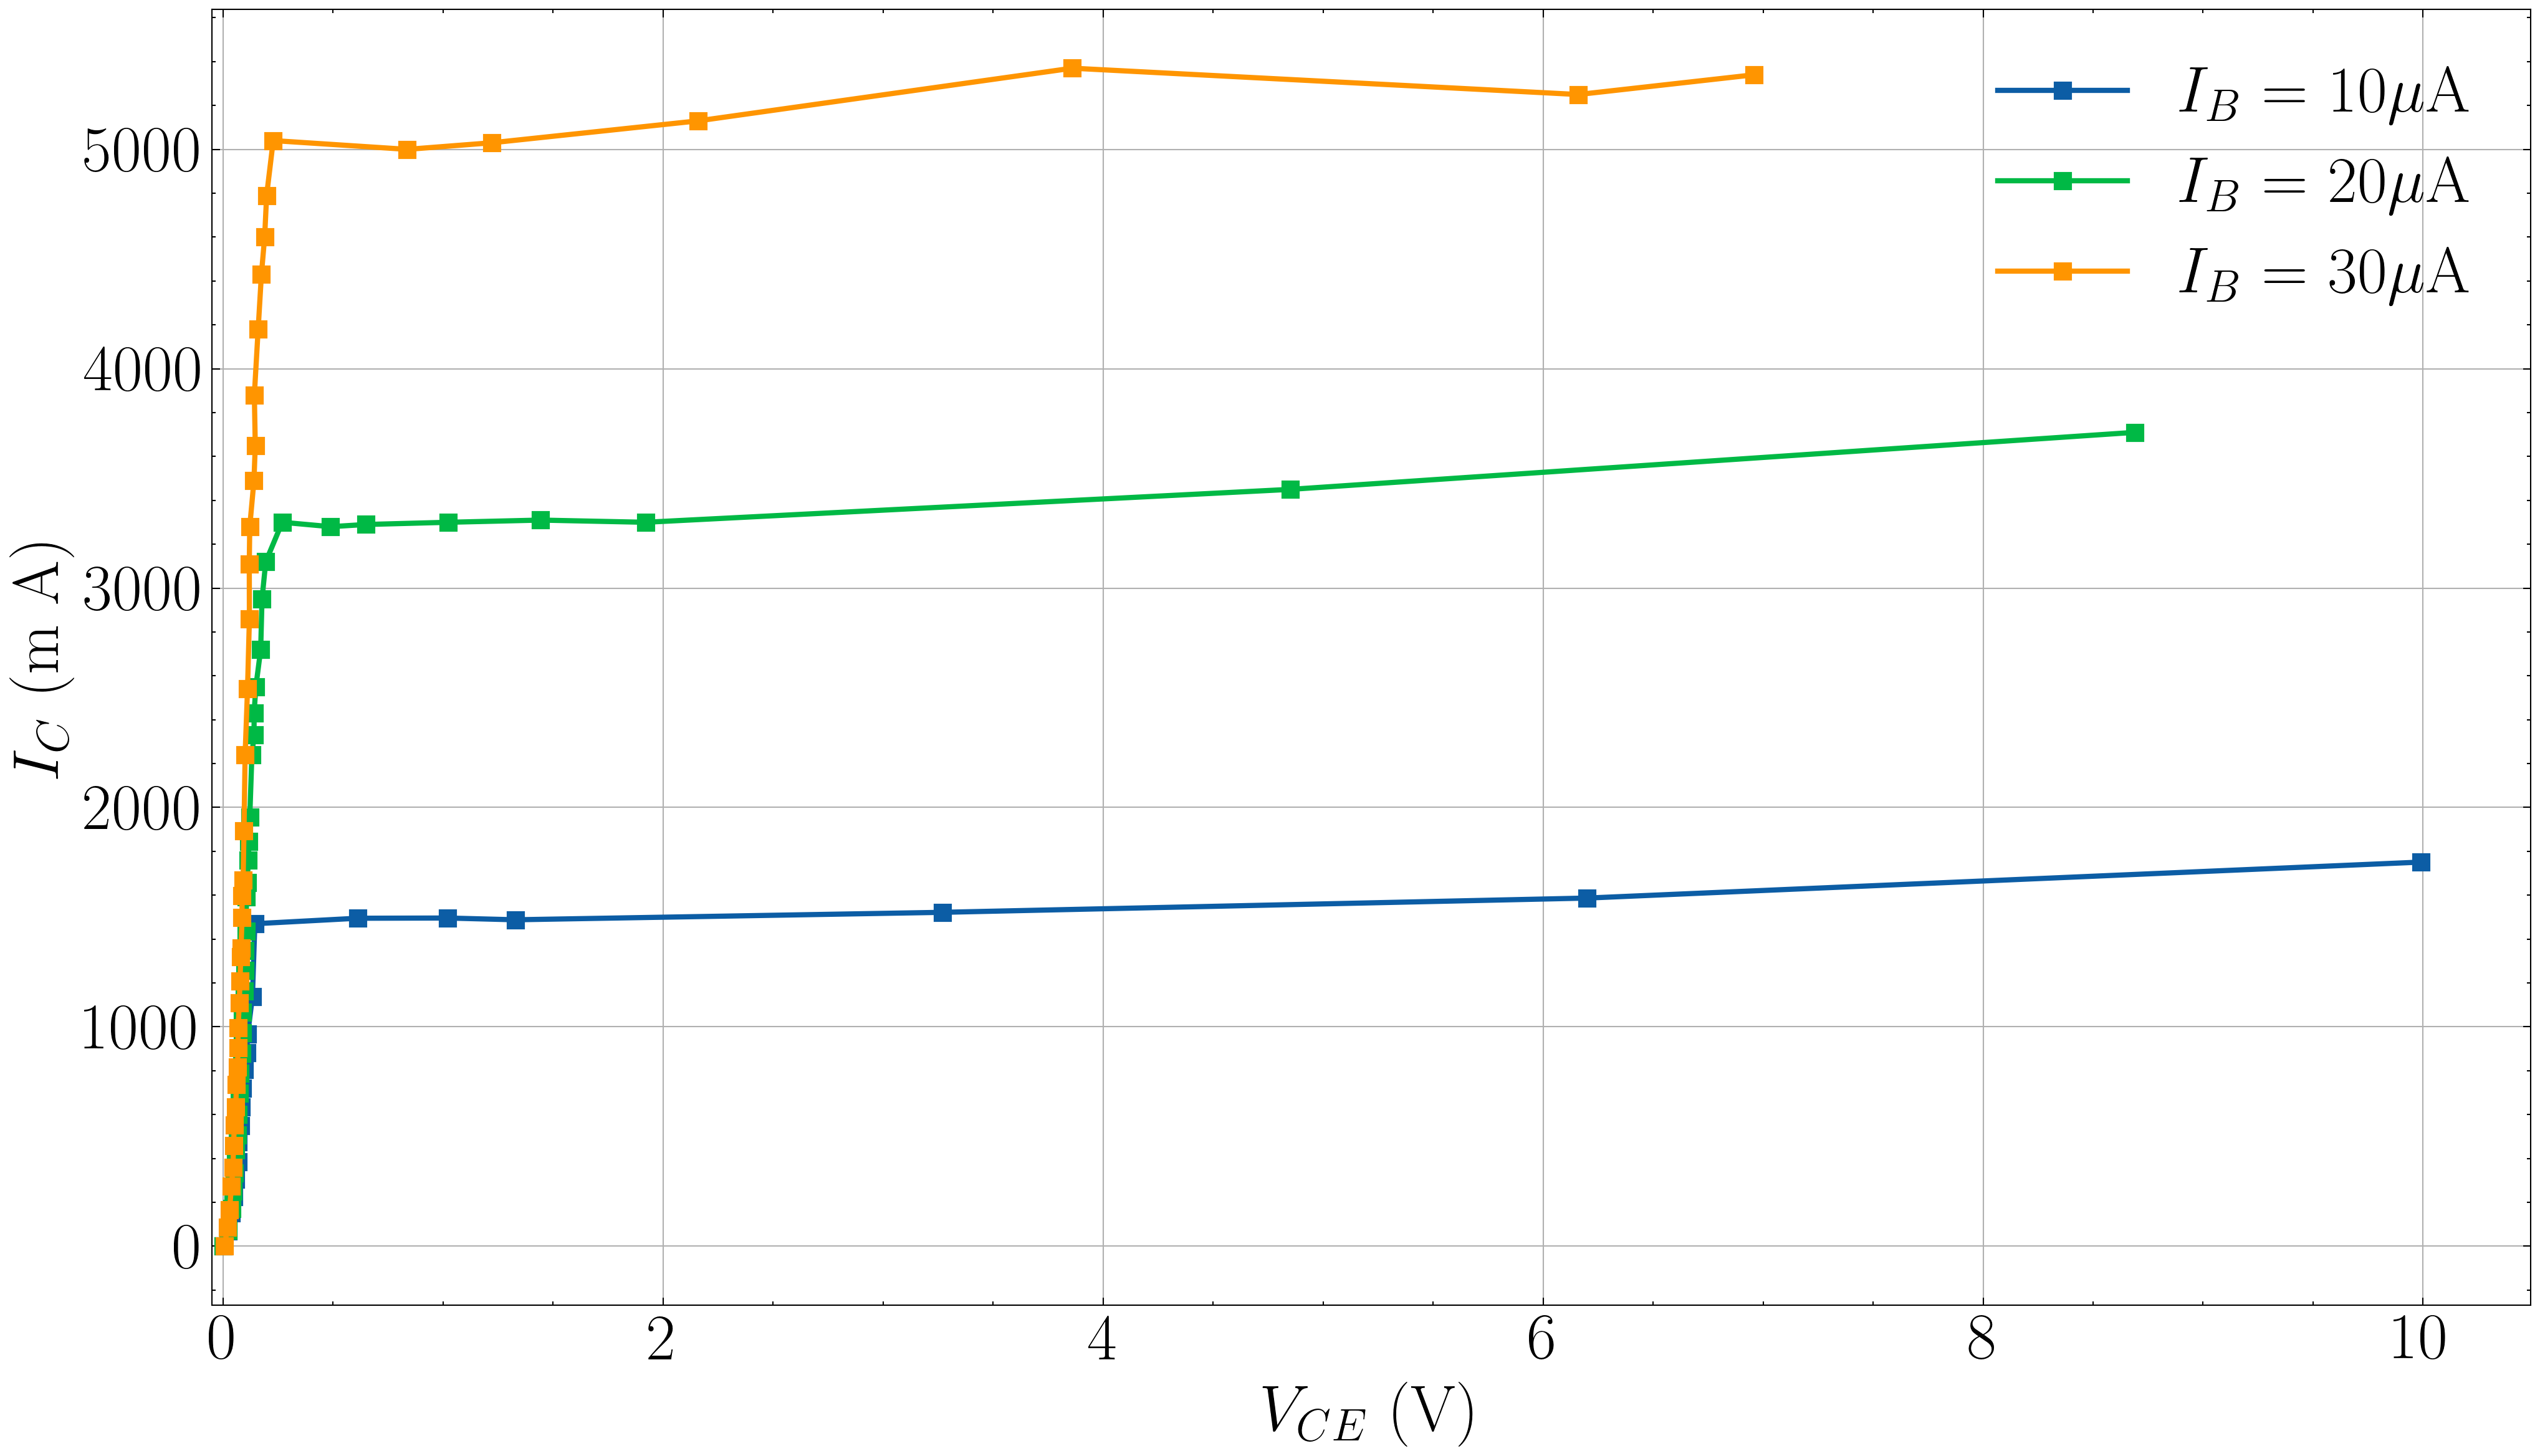
\includegraphics[width=0.75\textwidth]{output.png}
        \caption{Output Characteristics of an npn BJT}
\end{figure}
\section{Current gain of the BJT}
The current gain of the BJT is given by the formula:
\begin{equation}
        \beta = \frac{I_c}{I_b}
\end{equation}
We plot $I_c$ vs $I_b$ which we obtained for the input characteristics. We then take a linear fit to find the slope and ultimately we get the average 
value of $\beta$ for different $V_{BB}$. The $\beta$ values are given below as $\beta_{V_{BB}}$,
\begin{align}
        \beta_{2V} &= 131.2 \pm 0.31 \\
        \beta_{3V} &= 195 \pm 2.6\\
        \beta_{4V} &= 205 \pm 3.6
\end{align}
\begin{figure}[H]
        \centering
        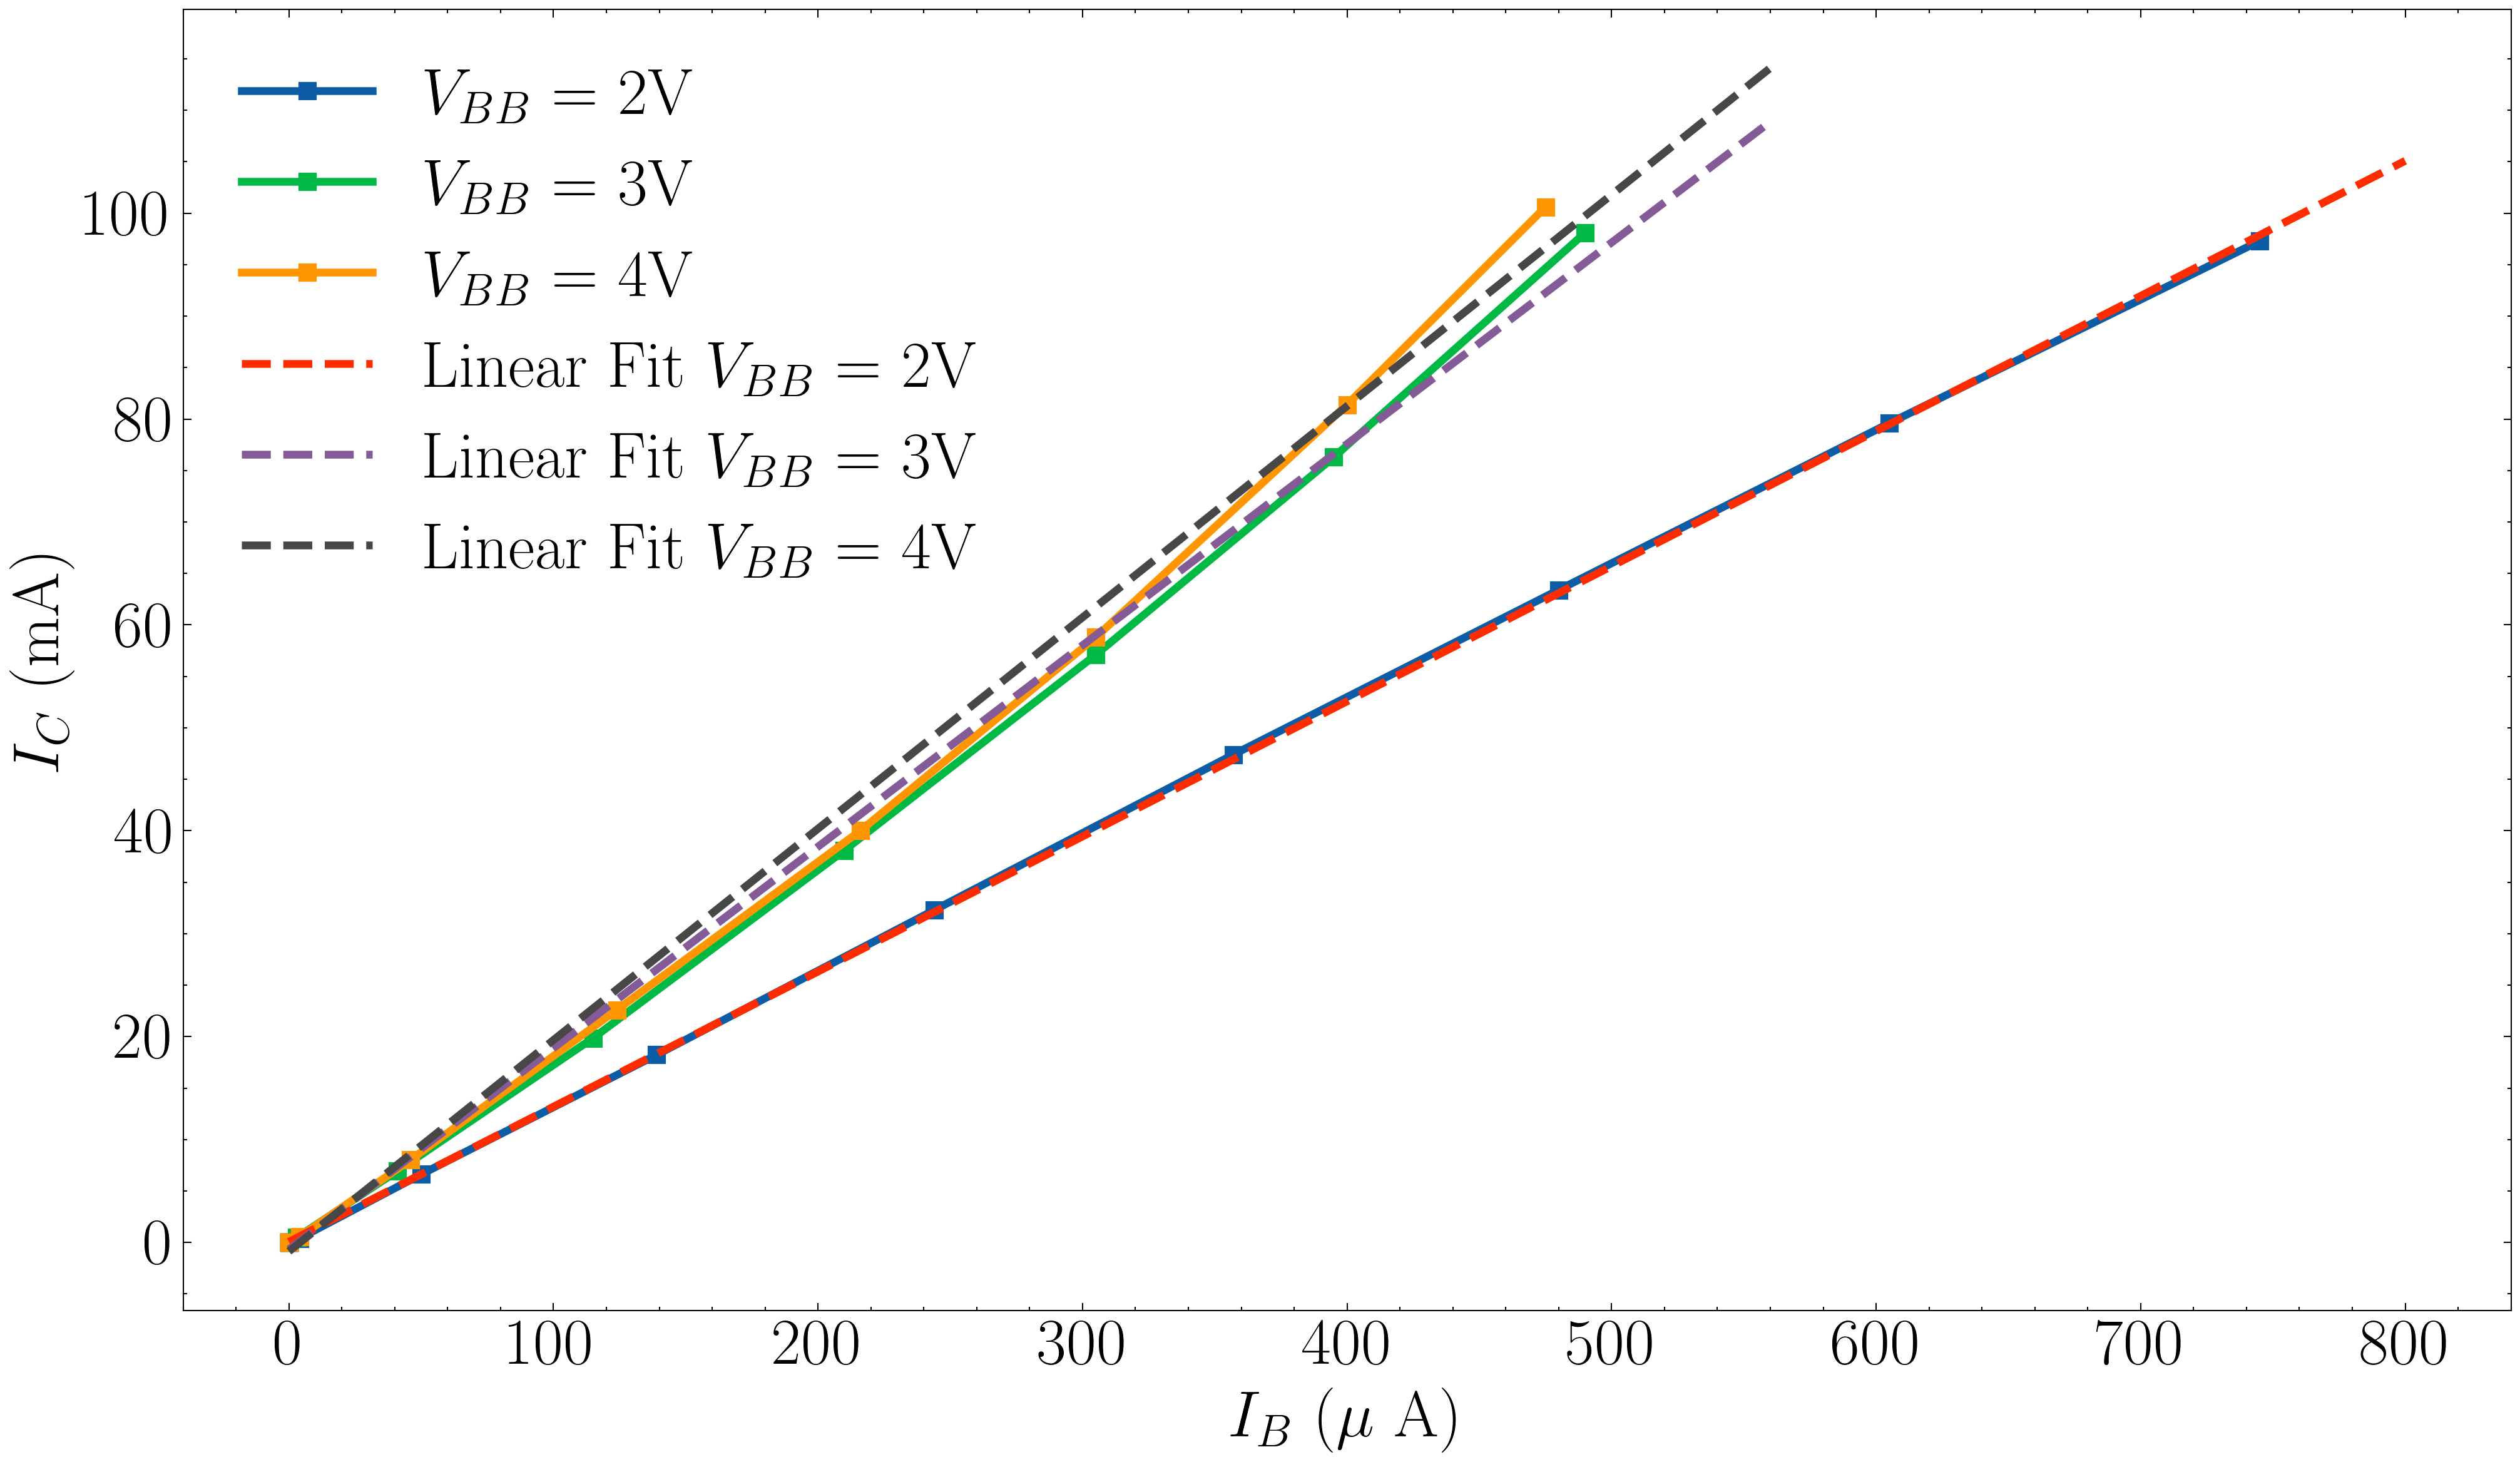
\includegraphics[width=0.75\textwidth]{beta.png}
        \caption{Current Gain of the BJT}
\end{figure}
\section{Results}
We have plotted the input and output characteristics with a small experimental anomaly. The current gain of the BJT is found to be $\beta_{2V} = 131.2 \pm 0.31, \beta_{3V} = 195 \pm 2.6, \beta_{4V} = 205 \pm 3.6$, which 
as expected, is quite large. 
\section{Sources of Error}
\begin{itemize}
        \item For the output characteristics, $I_b$ was fluctuating a lot , so the values are correct upto $\pm 3$ in the corresponding units.
        \item There are room temperature fluctuations which can affect the readings.
        \item As always, the least counts of the multimeters are a source of error.
        \item The source has voltage fluctuations which can affect the readings.
\end{itemize}
\section{Conclusion}
We conclude the experiment by finding the input and output characteristics of the BJT and also the current gain of the BJT from the input characteristics. The current gain is found to be quite large, as expected.
\pagebreak
\section{Supplementary}
\label{sec:supplementary}
\begin{table}[!ht]
        \centering
        \begin{tabular}{|l|l|l|l|l|l|}
        \hline
            \textbf{V\_BB} & \textbf{V\_BE} & \textbf{I\_b ($\mu A$)} & \textbf{I\_c( mA)} & \textbf{V\_CC} & \textbf{V\_CE} \\ \hline
            0 & 0 & 0 & 0 & 2 & 2 \\ \hline
            0.1 & 0.1232 & 0 & 0 & 2 & 2 \\ \hline
            0.2 & 0.234 & 0 & 0 & 2 & 2 \\ \hline
            0.4 & 0.458 & 0 & 0.007 & 2 & 2 \\ \hline
            0.5 & 0.564 & 4 & 0.4 & 2 & 2 \\ \hline
            0.6 & 0.639 & 50 & 6.62 & 2 & 2 \\ \hline
            0.7 & 0.674 & 139 & 18.23 & 2 & 2 \\ \hline
            0.8 & 0.696 & 244 & 32.3 & 2 & 2 \\ \hline
            0.9 & 0.721 & 357 & 47.4 & 2 & 2 \\ \hline
            1 & 0.745 & 480 & 63.4 & 2 & 2 \\ \hline
            1.1 & 0.769 & 605 & 79.6 & 2 & 2 \\ \hline
            1.2 & 0.781 & 745 & 97.3 & 2 & 2 \\ \hline
        \end{tabular}
        \caption{BJT Input Characteristics at $V_{CC} = 2V$}
        \label{tab:input2v}
    \end{table}

    \begin{table}[!ht]
        \centering
        \begin{tabular}{|l|l|l|l|l|l|}
        \hline
            \textbf{V\_BB} & \textbf{V\_BE} & \textbf{I\_b ($\mu A$)} & \textbf{I\_c( mA)} & \textbf{V\_CC} & \textbf{V\_CE} \\ \hline
            0 & 0 & 0 & 0 & 3 & 3 \\ \hline
            0.1 & 0.1156 & 0 & 0 & 3 & 3 \\ \hline
            0.2 & 0.236 & 0 & 0 & 3 & 3 \\ \hline
            0.3 & 0.343 & 0 & 0 & 3 & 3 \\ \hline
            0.4 & 0.462 & 0 & 6.00E-03 & 3 & 3 \\ \hline
            0.5 & 0.569 & 3 & 4.88E-01 & 3 & 3 \\ \hline
            0.6 & 0.639 & 41 & 6.95 & 3 & 3 \\ \hline
            0.7 & 0.669 & 115 & 19.86 & 3 & 3 \\ \hline
            0.8 & 0.683 & 210 & 38.1 & 3 & 3 \\ \hline
            0.9 & 0.689 & 305 & 57.1 & 3 & 3 \\ \hline
            1 & 0.696 & 395 & 76.3 & 3 & 3 \\ \hline
            1.1 & 0.709 & 490 & 98.1 & 3 & 3 \\ \hline
            1.2 & 0.787 & 530 & 111.2 & 3 & 3 \\ \hline
        \end{tabular}
        \caption{BJT Input Characteristics at $V_{CC} = 3V$}
        \label{tab:input3v}
    \end{table}

    \begin{table}[!ht]
        \centering
        \begin{tabular}{|l|l|l|l|l|l|}
        \hline
            \textbf{V\_BB} & \textbf{V\_BE} & \textbf{I\_b ($\mu A$)} & \textbf{I\_c( mA)} & \textbf{V\_CC} & \textbf{V\_CE} \\ \hline
            0 & 0 & 0 & 0 & 4 & 4 \\ \hline
            0.1 & 0.115 & 0 & 0 & 4 & 4 \\ \hline
            0.2 & 0.24 & 0 & 0 & 4 & 4 \\ \hline
            0.3 & 0.345 & 0 & 0 & 4 & 4 \\ \hline
            0.4 & 0.46 & 0 & 0.01 & 4 & 4 \\ \hline
            0.5 & 0.567 & 4 & 0.556 & 4 & 4 \\ \hline
            0.6 & 0.642 & 46 & 8.03 & 4 & 4 \\ \hline
            0.7 & 0.667 & 124 & 22.6 & 4 & 4 \\ \hline
            0.8 & 0.682 & 216 & 40 & 4 & 4 \\ \hline
            0.9 & 0.697 & 305 & 58.8 & 4 & 4 \\ \hline
            1 & 0.703 & 400 & 81.4 & 4 & 4 \\ \hline
            1.1 & 0.724 & 475 & 100.6 & 4 & 4 \\ \hline
        \end{tabular}
        \caption{BJT Input Characteristics at $V_{CC} = 4V$}
        \label{tab:input4v}
    \end{table}

    \begin{table}[!ht]
        \centering
        \begin{tabular}{|l|l|l|l|l|}
        \hline
            \textbf{V\_BB} & \textbf{I\_b ($\mu A$)} & \textbf{I\_c( $\mu A$)} & \textbf{V\_CC} & \textbf{V\_CE} \\ \hline
            0.44 & 10 & 0 & 0 & 0 \\ \hline
            0.46 & 10 & 70 & 0.1 & 0.0233 \\ \hline
            0.47 & 10 & 151 & 0.2 & 0.0367 \\ \hline
            0.47 & 10 & 226 & 0.3 & 0.0489 \\ \hline
            0.48 & 10 & 305 & 0.4 & 0.0584 \\ \hline
            0.5 & 10 & 385 & 0.5 & 0.0682 \\ \hline
            0.49 & 10 & 477 & 0.6 & 0.0677 \\ \hline
            0.49 & 10 & 549 & 0.7 & 0.0798 \\ \hline
            0.49 & 10 & 635 & 0.8 & 0.0837 \\ \hline
            0.49 & 10 & 720 & 0.89 & 0.0878 \\ \hline
            0.49 & 10 & 805 & 1 & 0.0978 \\ \hline
            0.5 & 10 & 882 & 1.1 & 0.1075 \\ \hline
            0.5 & 10 & 968 & 1.2 & 0.1122 \\ \hline
            0.5 & 10 & 1137 & 1.4 & 0.1335 \\ \hline
            0.51 & 10 & 1470 & 1.8 & 0.1444 \\ \hline
            0.51 & 10 & 1495 & 2.3 & 0.611 \\ \hline
            0.51 & 10 & 1.50E+03 & 2.7 & 1.021 \\ \hline
            0.51 & 10 & 1.49E+03 & 3 & 1.328 \\ \hline
            0.5 & 10 & 1522 & 4.98 & 3.27 \\ \hline
            0.5 & 10 & 1587 & 8 & 6.2 \\ \hline
            0.5 & 10 & 1751 & 11.97 & 9.99 \\ \hline
        \end{tabular}
        \caption{BJT Output Characteristics at $I_b$ = 10 $\mu A$}
        \label{tab:output10}
    \end{table}
    \begin{table}[!ht]
        \centering
        \begin{tabular}{|l|l|l|l|l|}
        \hline
            \textbf{V\_BB} & \textbf{I\_b ($\mu A$)} & \textbf{I\_c( $\mu A$)} & \textbf{V\_CC} & \textbf{V\_CE} \\ \hline
            0.47 & 20 & 0 & 0 & 0 \\ \hline
            0.49 & 20 & 72 & 0.1 & 0.0243 \\ \hline
            0.5 & 20 & 173 & 0.22 & 0.0393 \\ \hline
            0.5 & 20 & 251 & 0.31 & 0.0452 \\ \hline
            0.51 & 20 & 333 & 0.4 & 0.052 \\ \hline
            0.51 & 20 & 440 & 0.52 & 0.0562 \\ \hline
            0.52 & 20 & 508 & 0.6 & 0.0653 \\ \hline
            0.52 & 20 & 602 & 0.7 & 0.0686 \\ \hline
            0.52 & 20 & 696 & 0.8 & 0.0749 \\ \hline
            0.53 & 20 & 788 & 0.9 & 0.0781 \\ \hline
            0.53 & 20 & 878 & 1 & 0.0862 \\ \hline
            0.53 & 20 & 974 & 1.09 & 0.0876 \\ \hline
            0.53 & 20 & 1067 & 1.19 & 0.0894 \\ \hline
            0.53 & 20 & 1162 & 1.3 & 0.0955 \\ \hline
            0.53 & 20 & 1258 & 1.4 & 0.0997 \\ \hline
            0.53 & 20 & 1349 & 1.49 & 0.1004 \\ \hline
            0.53 & 20 & 1437 & 1.59 & 0.1051 \\ \hline
            0.54 & 20 & 1593 & 1.74 & 0.1063 \\ \hline
            0.54 & 20 & 1657 & 1.82 & 0.1102 \\ \hline
            0.54 & 20 & 1761 & 1.92 & 0.1146 \\ \hline
            0.54 & 20 & 1846 & 2 & 0.1179 \\ \hline
            0.54 & 20 & 1955 & 2.11 & 0.1214 \\ \hline
            0.54 & 20 & 2240 & 2.22 & 0.131 \\ \hline
            0.54 & 20 & 2330 & 2.32 & 0.141 \\ \hline
            0.54 & 20 & 2430 & 2.41 & 0.141 \\ \hline
            0.54 & 20 & 2550 & 2.52 & 0.149 \\ \hline
            0.54 & 20 & 2720 & 2.7 & 0.171 \\ \hline
            0.54 & 20 & 2950 & 2.9 & 0.177 \\ \hline
            0.54 & 20 & 3120 & 3.08 & 0.194 \\ \hline
            0.54 & 20 & 3300 & 3.33 & 0.269 \\ \hline
            0.54 & 20 & 3280 & 3.53 & 0.489 \\ \hline
            0.54 & 20 & 3290 & 3.7 & 0.65 \\ \hline
            0.54 & 20 & 3300 & 4.07 & 1.023 \\ \hline
            0.54 & 20 & 3310 & 4.5 & 1.443 \\ \hline
            0.54 & 20 & 3300 & 5 & 1.92 \\ \hline
            0.54 & 20 & 3450 & 8.05 & 4.85 \\ \hline
            0.54 & 20 & 3710 & 12.11 & 8.69 \\ \hline
        \end{tabular}
        \caption{BJT Output Characteristics at $I_b$ = 20 $\mu A$}
        \label{tab:output20}
    \end{table}

    \begin{table}[!ht]
    \centering
    \begin{tabular}{|l|l|l|l|l|}
    \hline
        \textbf{V\_BB} & \textbf{I\_b ($\mu A$)} & \textbf{I\_c( $\mu$ A)} & \textbf{V\_CC} & \textbf{V\_CE} \\ \hline
        0.47 & 30 & 0 & 0 & 0.0069 \\ \hline
        0.48 & 30 & 87 & 0.1 & 0.0202 \\ \hline
        0.49 & 30 & 167 & 0.2 & 0.0295 \\ \hline
        0.49 & 30 & 274 & 0.31 & 0.0382 \\ \hline
        0.5 & 30 & 358 & 0.4 & 0.0451 \\ \hline
        0.51 & 30 & 459 & 0.51 & 0.0472 \\ \hline
        0.51 & 30 & 551 & 0.61 & 0.0516 \\ \hline
        0.51 & 30 & 634 & 0.7 & 0.0581 \\ \hline
        0.51 & 30 & 737 & 0.8 & 0.0603 \\ \hline
        0.51 & 30 & 818 & 0.89 & 0.0662 \\ \hline
        0.51 & 30 & 904 & 0.99 & 0.0675 \\ \hline
        0.52 & 30 & 997 & 1.08 & 0.0686 \\ \hline
        0.52 & 30 & 1108 & 1.2 & 0.0735 \\ \hline
        0.52 & 30 & 1209 & 1.3 & 0.0771 \\ \hline
        0.52 & 30 & 1319 & 1.42 & 0.0803 \\ \hline
        0.53 & 30 & 1358 & 1.47 & 0.0815 \\ \hline
        0.53 & 30 & 1499 & 1.61 & 0.0865 \\ \hline
        0.53 & 30 & 1599 & 1.71 & 0.0861 \\ \hline
        0.53 & 30 & 1669 & 1.78 & 0.0911 \\ \hline
        0.53 & 30 & 1894 & 2.02 & 0.0951 \\ \hline
        0.53 & 30 & 2240 & 2.19 & 0.1002 \\ \hline
        0.54 & 30 & 2540 & 2.48 & 0.1112 \\ \hline
        0.54 & 30 & 2860 & 2.8 & 0.1197 \\ \hline
        0.54 & 30 & 3110 & 3.04 & 0.1191 \\ \hline
        0.54 & 30 & 3280 & 3.21 & 0.1213 \\ \hline
        0.54 & 30 & 3490 & 3.42 & 0.1404 \\ \hline
        0.54 & 30 & 3650 & 3.62 & 0.1464 \\ \hline
        0.54 & 30 & 3880 & 3.79 & 0.1422 \\ \hline
        0.55 & 30 & 4180 & 4.09 & 0.1595 \\ \hline
        0.55 & 30 & 4430 & 4.33 & 0.1743 \\ \hline
        0.55 & 30 & 4600 & 4.5 & 0.189 \\ \hline
        0.55 & 30 & 4790 & 4.71 & 0.198 \\ \hline
        0.55 & 30 & 5040 & 4.94 & 0.228 \\ \hline
        0.55 & 30 & 5000 & 5.53 & 0.837 \\ \hline
        0.55 & 30 & 5030 & 5.97 & 1.221 \\ \hline
        0.55 & 30 & 5130 & 7.02 & 2.16 \\ \hline
        0.55 & 30 & 5370 & 8.96 & 3.86 \\ \hline
        0.55 & 30 & 5250 & 11.13 & 6.16 \\ \hline
        0.55 & 30 & 5340 & 11.98 & 6.96 \\ \hline
    \end{tabular}
    \caption{BJT Output Characteristics at $I_b$ = 30 $\mu A$}
    \label{tab:output30}
\end{table}
\end{document}
